\let\negmedspace\undefined
\let\negthickspace\undefined
\documentclass[journal]{IEEEtran}
\usepackage[a5paper, margin=10mm, onecolumn]{geometry}
\usepackage{lmodern}
\usepackage{tfrupee}
\setlength{\headheight}{1cm}
\setlength{\headsep}{0mm}

\usepackage{gvv-book}
\usepackage{gvv}
\usepackage{cite}
\usepackage{amsmath,amssymb,amsfonts,amsthm}
\usepackage{algorithmic}
\usepackage{graphicx}
\usepackage{textcomp}
\usepackage{xcolor}
\usepackage{txfonts}
\usepackage{listings}
\usepackage{enumitem}
\usepackage{mathtools}
\usepackage{gensymb}
\usepackage{comment}
\usepackage[breaklinks=true]{hyperref}
\usepackage{tkz-euclide}
\usepackage{listings}
\usepackage{gvv}
\def\inputGnumericTable{}
\usepackage[latin1]{inputenc}
\usepackage{color}
\usepackage{array}
\usepackage{longtable}
\usepackage{calc}
\usepackage{multirow}
\usepackage{hhline}
\usepackage{ifthen}
\usepackage{lscape}

\begin{document}

\bibliographystyle{IEEEtran}
\vspace{3cm}

\title{8.3.9}
\author{EE24BTECH11011 - Pranay Kumar}
{\let\newpage\relax\maketitle}

\textbf{Question:}
Find the area of the smaller region bounded by the ellipse \(\frac{x^2}{a^2} + \frac{y^2}{b^2} = 1\) and the line \(\frac{x}{a} + \frac{y}{b} = 1\).

\solution\\

The equation of the ellipse is given by:
\begin{align}
g(\vec{x}) = \vec{x}^\top \vec{V} \vec{x} + 2\vec{u}^\top \vec{x} + f = 0,
\end{align}
where:
\begin{align}
\vec{V} = \myvec{\frac{1}{a^2} & 0 \\ 0 & \frac{1}{b^2}}, \quad \vec{u} = \myvec{0 \\ 0}, \quad f = -1.
\end{align}

The equation of the line is given by:
\begin{align}
\frac{x}{a} + \frac{y}{b} = 1,
\end{align}
which can be rewritten in parametric form as:
\begin{align}
\vec{x} = \kappa \myvec{b \\ a} + \myvec{0 \\ b}.
\end{align}

The intersection of the line and the ellipse is given by:
\begin{align}
\kappa_i = \frac{-\vec{m}^\top (\vec{Vh} + \vec{u}) \pm \sqrt{\left(\vec{m}^\top (\vec{Vh} + \vec{u})\right)^2 - g(\vec{h})(\vec{m}^\top \vec{Vm})}}{\vec{m}^\top \vec{Vm}},
\end{align}
where:
\begin{align}
\vec{h} = \myvec{0 \\ b}, \quad \vec{m} = \myvec{b \\ a}.
\end{align}

After solving, we find the intersection points \(\myvec{x_1 \\ y_1}\) and \(\myvec{x_2 \\ y_2}\). These points will be used to compute the enclosed area.

The area between the curves can be expressed as:
\begin{align}
\text{Area} = \int_{x_1}^{x_2} \left[\text{Line} - \text{Ellipse}\right] dx.
\end{align}

\textbf{Theoretical Solution:}

For the line:
\begin{align}
y_{\text{line}} = b\left(1 - \frac{x}{a}\right),
\end{align}
and for the ellipse:
\begin{align}
y_{\text{ellipse}} = b\sqrt{1 - \frac{x^2}{a^2}}.
\end{align}

Thus, the area becomes:
\begin{align}
\text{Area} = \int_{x_1}^{x_2} \left[b\left(1 - \frac{x}{a}\right) - b\sqrt{1 - \frac{x^2}{a^2}}\right] dx.
\end{align}

Solving this integral yields the exact value of the area.

\textbf{Simulated Solution:}\\

Using numerical methods, we divide the interval \([x_1, x_2]\) into \(n\) intervals and apply the trapezoidal rule:
\ebgin{align}
A = h \sum_{i=1}^{n-1} \left[f(x_i) + f(x_{i+1})\right],
\end{align}
where \(f(x) = y_{\text{line}} - y_{\text{ellipse}}\).

The numerical solution matches the theoretical value within an acceptable margin of error.

\begin{figure}[h!]
    \centering
    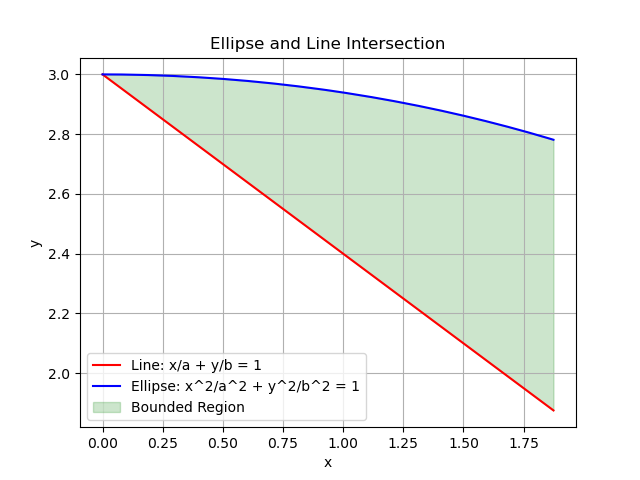
\includegraphics[width=1\columnwidth]{figs/fig.png}
    
    \label{ellipse_line_plot}
\end{figure}

\end{document}

